This whole procedure that we discussed in the previous section, helped us to successfully converted each image of the video that contains only a single person into an array that contains the 3D pose estimation of a human. However, we still are missing something. What we need is the 6D human pose estimation. At this moment we have the knowledge of the orientation of each human bone that our humanoid skeleton has. We have to find the location of the humanoid in the space, which is important if the user wants to apply the root motion to his avatar. A mocap suit estimates the position of each bone in the space, so if we need to match the quality of it we should do the same. However, in our case, the best option was to estimate the location of the parent bone of the human (the hip) and move into space the humanoid according to the hip location. Imagine that our human is moving like a marionette, it can rotate each bone of the body, but the location of the marionette will be according to the actor's hand that is controlling it.\\

Therefore, we came up with a solution to this problem that would help us estimate the human location from a single image. We can use some knowledge that we already have from our models. More specifically, the first model, the 2D human pose estimator, predicts 17 keypoints of the human skeleton, as we have already shown in a figure in the previous sections. In order to estimate the (x,y) of the position we will find the average pixel in the image, between these 17 keypoints. If we do so, this point location should be estimating the human hip position as it is shown in the figure below.

\pagebreak

\begin{figure}[h]
	\centering
	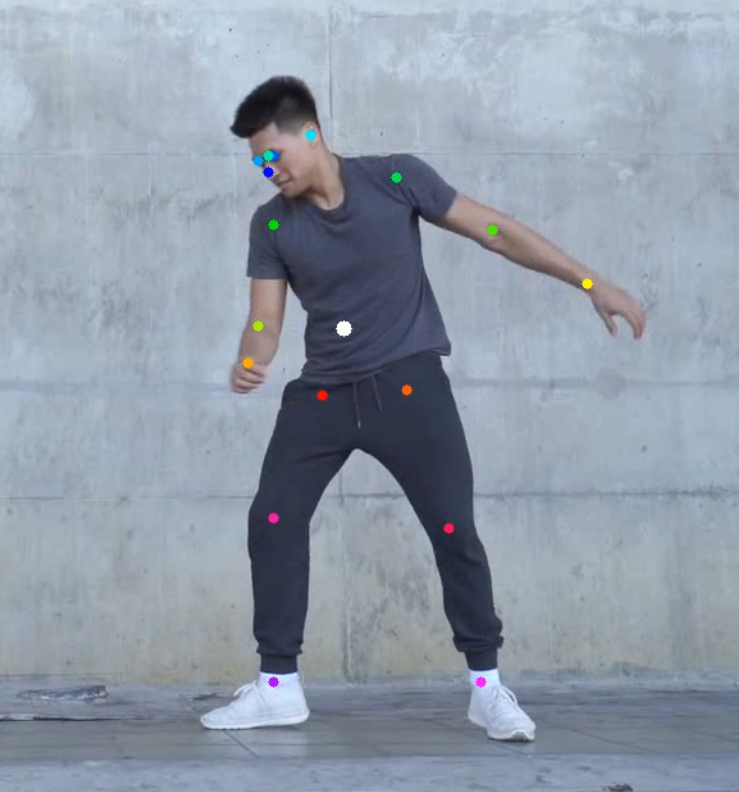
\includegraphics[width=0.65\textwidth]{figures/Implementation/position2D.png}
	\captionsetup{labelformat=empty}
	\caption{\href{https://www.pexels.com/search/videos/dance/}
	{The multi-color keypoints represent the 17 keypoints that the AlphaPose model estimated . The white keypoint is the average of all the estimated keypoints which we will use as the 2D location of the humanoid.}}
\end{figure}

However, we still are missing the Z dimension of the position. Estimating the Depth from a single image is something that many researchers try to solve.Some state-of-the-art works can estimate the 3D location of an object from an image with great accuracy. The most accurate method is to use two cameras to take the image of the object from two different positions. This would minimize the depth error estimation. However, we did not choose this method because it requires two cameras, but we decided to convert the motion of a human from a single video, we wanted our algorithm to be as simpler as it can get for the user.\\

Therefore, the solution that we came up with is very fast O(N) (N is the number of the frames from the input video), but the accuracy in some cases is not great. Again, using the 17 keypoints of the AlphaPose model, we segmented the human inside a box, that contains all the keypoints. In order to estimate the depth of the image, we calculate the $log(area)_2$ of this box, and we normalize this number depending on the video resolution. Due to the log, small changes due to some limb motion do not affect the results. The animators can fix some errors in the humanoid position later, but we will also offer a tool that will help them in this procedure. In the figure below we can the human box segmentation.

\begin{figure}[h]
	\centering
	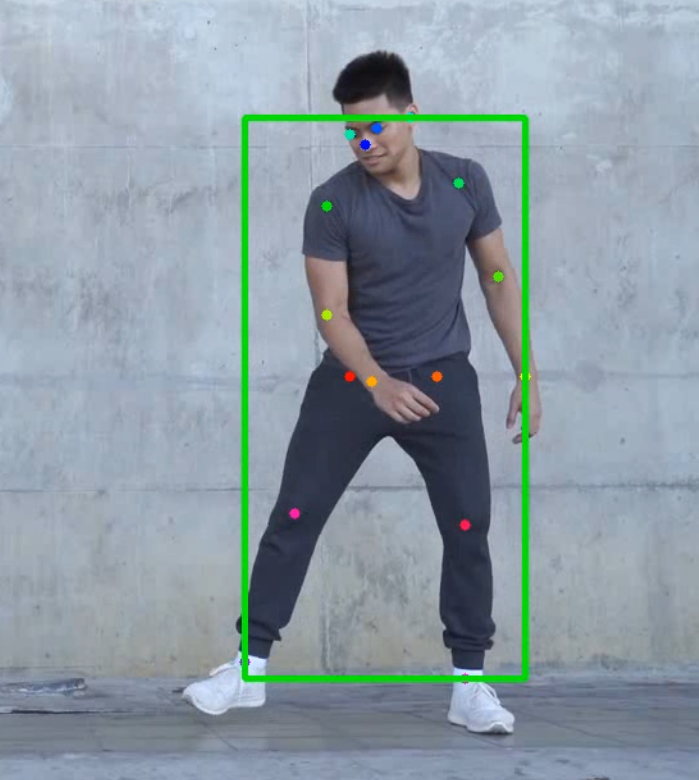
\includegraphics[width=0.65\textwidth]{figures/Implementation/position3D.png}
	\captionsetup{labelformat=empty}
	\caption{\href{https://www.pexels.com/search/videos/dance/}
	{Human Segmentation using the 17 keypoints from AlphaPose model}}
\end{figure}

